% Source of the figure positions.pdf: the positions along the walk in the remaining case of the proof of the theorem on
% bounded formulas. The bars show the ranges of the positions of R_0 and C_0, the ticks the thresholds. The ends of the
% lower contacts of h and the upper contacts of a lie outside. The dark part of the bar of C_0 lies beyond tau^*, where
% every class of C_0 has a position. The tail starts after p^*. Compile with pdfLaTeX; included at its natural size.
\documentclass[tikz,border=1pt]{standalone}
\usepackage[T1]{fontenc}
\pdfinfoomitdate=1 \pdftrailerid{} \pdfsuppressptexinfo=-1
\usetikzlibrary{arrows.meta, decorations.pathreplacing}
\tikzset{
  axis/.style={line width=0.7pt, -{Stealth[length=2.4mm, width=2mm]}},
  tick/.style={line width=0.7pt},
  bar/.style={fill=gray!25, draw=gray!75!black, line width=0.6pt},
  darkbar/.style={fill=gray!60, draw=gray!75!black, line width=0.6pt},
  guide/.style={line width=0.4pt, gray!70, dash pattern=on 2pt off 2pt}}
\begin{document}
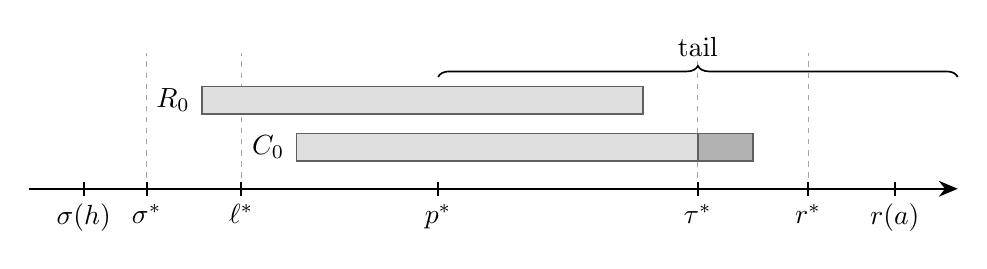
\begin{tikzpicture}[x=1cm, y=1cm]
  \def\ps{0.7} \def\ss{1.5} \def\ls{2.7} \def\ts{8.5} \def\rs{9.9} \def\pf{11.0} \def\m{0.7}
  % guides from the axis to the bars
  \foreach \x in {\ss,\ls,\ts,\rs} \draw[guide] (\x,0) -- (\x,1.72);
  % bars
  \draw[bar] (\ss+\m,0.95) rectangle (\ts-\m,1.3);
  \node[anchor=east] at (\ss+\m-0.03,1.125) {$R_0$};
  \draw[bar] (\ls+\m,0.35) rectangle (\rs-\m,0.7);
  \draw[darkbar] (\ts,0.35) rectangle (\rs-\m,0.7);
  \node[anchor=east] at (\ls+\m-0.03,0.525) {$C_0$};
  % axis and ticks
  \draw[axis] (0,0) -- (11.8,0);
  \foreach \x/\t in {\ps/{\sigma(h)},\ss/{\sigma^*},\ls/{\ell^*},\ts/{\tau^*},\rs/{r^*},\pf/{r(a)}} {
    \draw[tick] (\x,-0.09) -- (\x,0.09);
    \node[below=2pt] at (\x,0) {$\t$};
  }
  % the tail
  \def\pp{5.2}
  \draw[tick] (\pp,-0.09) -- (\pp,0.09);
  \node[below=2pt] at (\pp,0) {$p^*$};
  \draw[decorate, decoration={brace, amplitude=4pt}, line width=0.6pt] (\pp,1.42) -- (11.8,1.42);
  \node[above=4pt] at (8.5,1.42) {tail};
\end{tikzpicture}
\end{document}
